\documentclass[twocolumn]{article}
\usepackage{graphicx}
\title{ Assignment 1 \\ Computational Physics I - Physic 381 }
\author{Guilherme Contesini , 10140201 }

\begin{document}
\maketitle
\date
%%%%%%%%%%%%%%%%%%%%%%%%%%%%%%%%%%%%%%%%%%%%%%%%%%%%%%%%%%%%%%%%%%%%%%%%%%%%%%%%%%%%%%%%%%%%%%%%%%%%%%%%%%%%%%%%%%%%%%%%
\section{Introduction}
Part one:
\paragraph{}
Represent data is often challenging because each data set may have different interpretations, the most common way to plot a set of data is via the technique of plotting point by point according to their respective coordinates, however this technique is not useful for certain situations, as in the case of representing matrices, on this  report will be showed a matrix plot that for each value on the matrix will be used a different color.
%%%%%%%%%%%%%%%%%%%%%%%%%%%%%%%%%%%%%%%%%%%%%%%%%%%%%%%%%%%%%%%%%%%%%%%%%%%%%%%%%%%%%%%%%%%%%%%%%%%%%%%%%%%%%%%%%%%%%%%%
\section{Gnuplot:\\Visualizing matrices as 2-dimensional color maps}
\subsection{}
The matrix will appear reversed because Gnuplot plots the colors according to the coordinates provided then the table from Appendix A will be different from the final result generated by Gnuplot.The explanation of the code can be found in [~\ref{plotting first graphic}].
\begin{figure}[h!]
\begin{center}
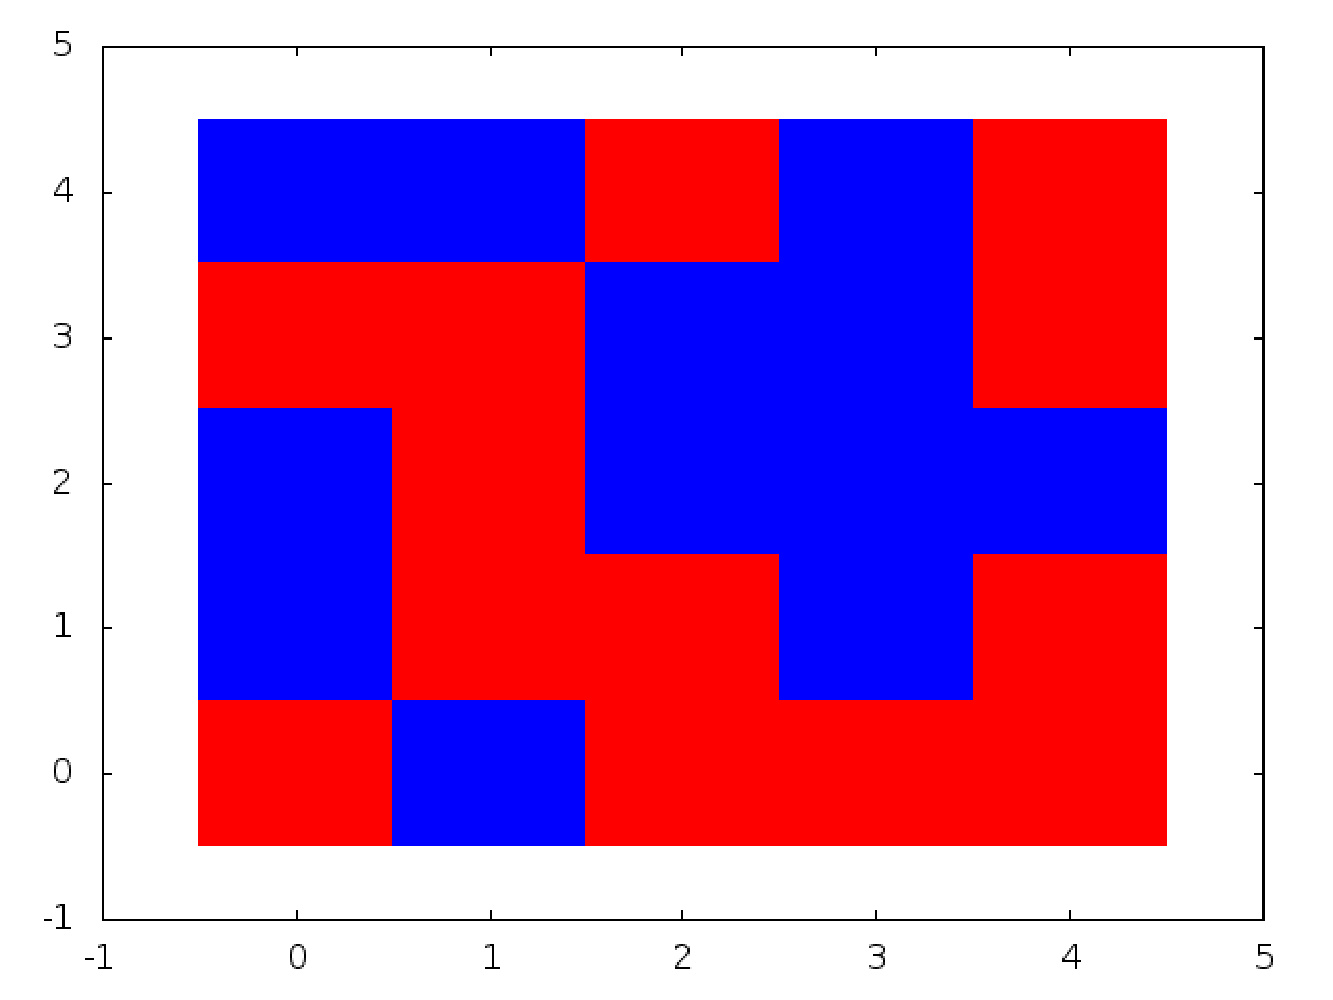
\includegraphics[width=2.1in]{fig1.pdf}
\caption{Color map Matrix}
\label{Color map Matrix}
\end{center}
\end{figure}
\subsection{}
The program written to generate matrices will be identical except for a few lines of code.
The lines that are different from each other are:
\begin{itemize}
\item The file name and the tag (12, file = "data2.txt"), where the tag and the name was changed.
\item The conditions within the IF statement. That define how the matrix will look like.
\end{itemize}
\subsubsection{(i):}
\paragraph{}
The condition for writing this matrix is to write 1 in the positions where the column is equal to the line, and where the sum of the index of the row with the index of the column is equal to the number of columns on matrix plus 1.The explanation of the code can be found in [~\ref{writing first matrix}].
\subsubsection{(ii):}
\paragraph{}
The condition for writing this matrix is to write 1 in the positions where the number column and line number are equal to half the number of columns, knowing that the matrix is quadratic. Note that for a even matrix  must be added a second condition where you need to write 1 in the positions where the number of the column and line number are equal to half the number of columns plus 1.The explanation of the code can be found in [~\ref{writing second matrix}].
\subsubsection{(iii):}
\paragraph{}
The condition to write this matrix is to write 1 in the positions when the column is equal to 1 and when it is equal to the number of columns, the same condition is used in relation the lines, whose line elements equals 1 and where is equal to the number lines.The explanation of the code can be found in [~\ref{writing third matrix}].
\subsubsection{(iv):}
\paragraph{}
The condition to write this matrix is to write 1 in the positions where the column and row are multiple of two.The explanation of the code can be found in [~\ref{writing fourth matrix}].
\subsection{}
The code for plotting this graphic can be found in [~\ref{four graphic screen}].

\begin{figure}[h!]
\begin{center}
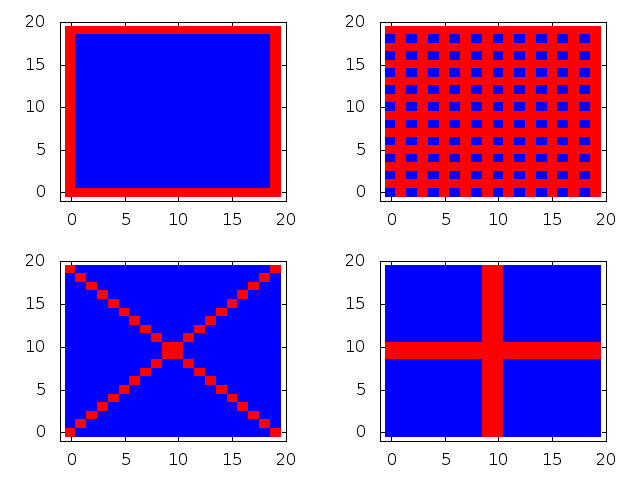
\includegraphics[width=3in]{fig2.png}
\caption{Four Matrix}
\label{Four Matrix}
\end{center}
\end{figure}
%%%%%%%%%%%%%%%%%%%%%%%%%%%%%%%%%%%%%%%%%%%%%%%%%%%%%%%%%%%%%%%%%%%%%%%%%%%%%%%%%%%%%%%%%%%%%%%%%%%%%%%%%%%%%%%%%%%%%%%%
\section{Astrophysics:\\Ultra-High Energy Cosmic Rays}

\subsection{}
\subsubsection{(i)}
\paragraph{}
A accelerated proton in UHECR is a hundred million times greater than what we can produce in Earth.
I guess that we could find accelerated protons with that energy in the interior of a star, or at places near a neutron star or black hole, where the energies involved are huge.
\subsection{(ii)}
The explanation of the code and the can be found in [~\ref{three graphics script}].

\begin{figure}[h!]
\begin{center}
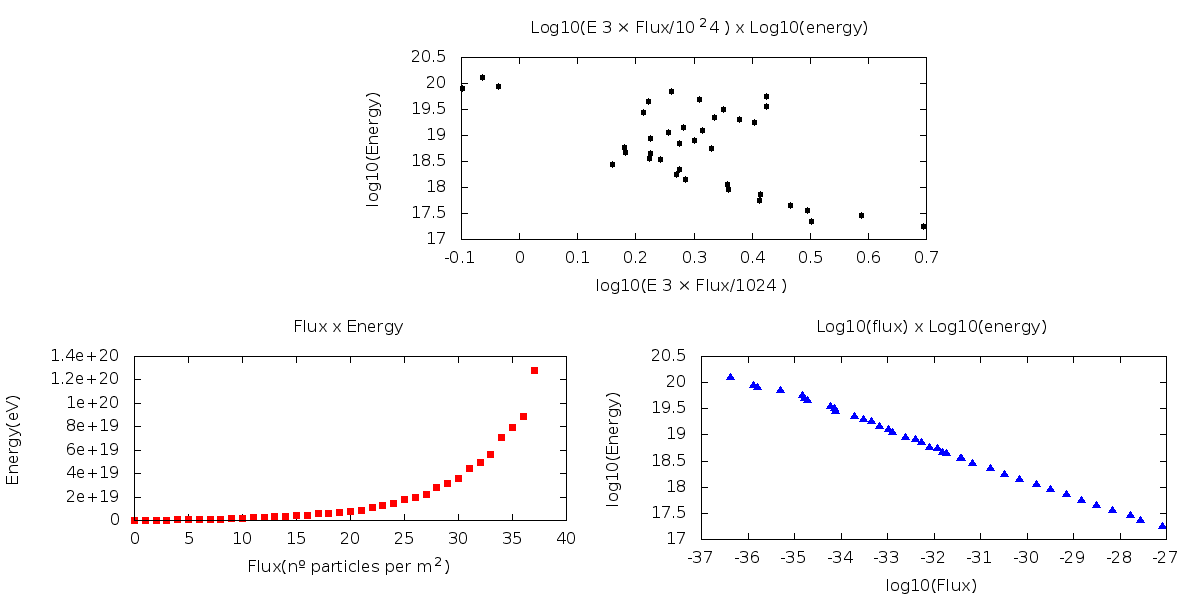
\includegraphics[width=3in]{fig3.png}
\caption{Three Graphics}
\label{Three Graphics.}
\emph{Note:The graphic flux $\times$ energy is on xlogscale.}
\end{center}
\end{figure}

\subsection{(iii)}
I suppose that the log10(E 3 × Flux/1024 ) versus log10(energy) graph because that shows that a for small and high energies you have a linear behaviour, but between those bands you have a strange behaviour.

\begin{figure}[h!]
\begin{center}
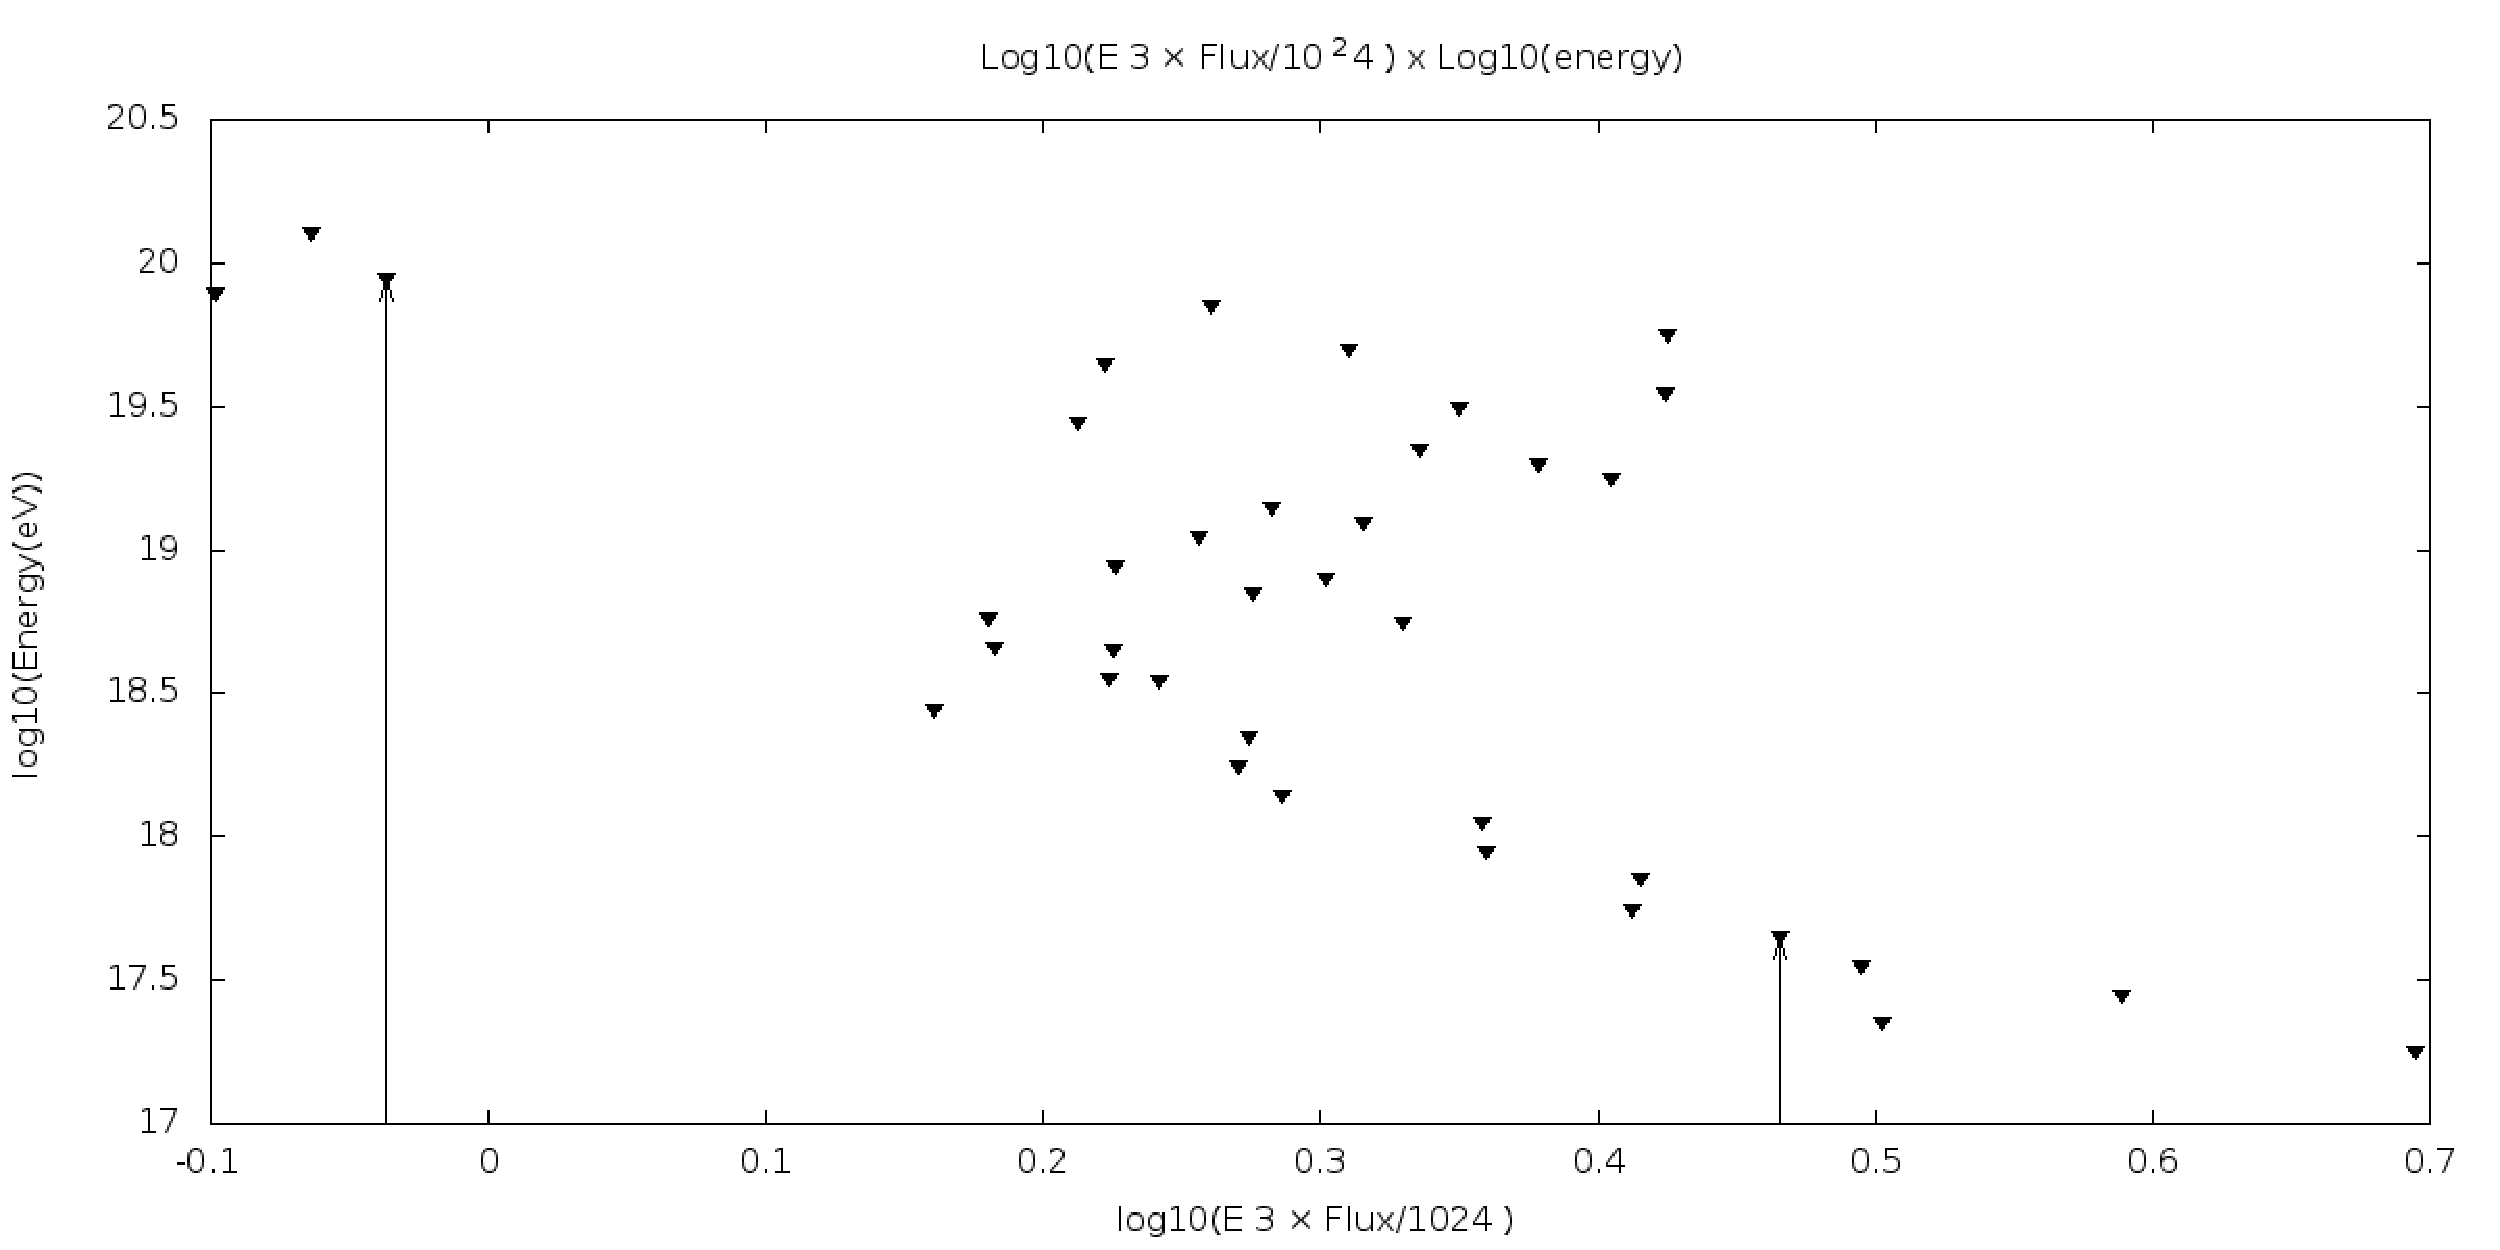
\includegraphics[width=3in]{fig4.pdf}
\caption{log10(E 3 × Flux/1024 ) $\times$ log10(energy)}
\label{}
\end{center}
\end{figure}
\newpage
\subsection{}
The E intersection between the regimes 1 and 2 is 3.13e18 and the intersection between regimes 2 and 3
is 2.52e19. If you give to the program the same input you will get a error saying that the program cannot compute a zero division, because in the formula you have $\frac{p_j}{p_i-p_j}$ and $\frac{p_i}{p_i-p_j}$.The explanation of the code for calculating the interception can be found in [~\ref{Fortran program for E}].\\
\\
\begin{tabular}{|l|l|l|l|l|}
\hline{}
reg.&Energy range(eV)&C&E_0&p \\\hline
1&1e17$<$E$<$3e18 & 5e-17&1.e17&-3.35\\\hline
2&3.1e18$<$E$<$2.5e19&5.5e-32&3e18&-2.79  \\\hline
3&2.5e19$<$E$<$1e21&1.5e-34&2.5e19&-3.49\\\hline 
\end{tabular}

%%%%%%%%%%%%%%%%%%%%%%%%%%%%%%%%%%%%%%%%%%%%%%%%%%%%%%%%%%%%%%%%%%%%%%%%%%%%%%%%%%%%%%%%%%%%%%%%%%%%%%%%%%%%%%%%%%%%%%%%
\section{Conclusion}
\paragraph{}
Using not very usual commands with those who we already know inside the graphical environment of Gnuplot, we saw that through this different method and with the proper numerical interpretation we can plot arrays and matrix with a more comprehensive manner and facilitating the final analysis of the initial data.
Also observed that the Fortran language can be used as a powerful tool to make systematic and complicated calculations that have several variables and require special attention in relation of the accuracy of the numbers.
%%%%%%%%%%%%%%%%%%%%%%%%%%%%%%%%%%%%%%%%%%%%%%%%%%%%%%%%%%%%%%%%%%%%%%%%%%%%%%%%%%%%%%%%%%%%%%%%%%%%%%%%%%%%%%%%%%%%%%%%
\section{Appendix Codes:}

\subsection{Part 1 codes:}

\subsubsection{Gnuplot script}

\begin{verbatim}
reset 
# reset all previously commands
set terminal gif
# say to gnuplot that all output 
file will be generate as .gif
 format
set output "fig1.gif"
# say to gnuplot that the output 
# will have the name 2Dmao.gif 
set palette maxcolors 2
# say to gnuplot to use only colors
unset colorbox
# say to gnuplot to don't plot the
# color box
set palette defined (0 'blue',
 1 'red')
# say to gnuplot to use color blue
 where is 0
# and color red where is 1
plot "data1.txt" matrix with image
 notitle
# plot the data inside "data1.txt"
 on a matrix way
# like a image with no title
!convert "fig1.gif" "fig1.pdf" && rm
 "fig1.gif"
# conver the output image from fig1.gif
 to fig1.pdf
# and remove the file fig1.gif
\end{verbatim}\label{plotting first graphic}

\subsubsection{Making a Matrix part(i):}

\begin{verbatim}
program matrix
  implicit none
  integer :: a , b, c, d
  a=1
  b=0
  print*, "Enter the x length of
   the matrix:"
  read(*,*) c
  print*, "Enter the y length of
   the matrix:"
  read(*,*) d
  call buildmatrix(a,b,c,d)
end program

subroutine buildmatrix(a,b,c,d)
  integer, intent(in) :: a,b,c,d
  integer, dimension(c,d) :: matrix
  integer :: i,j
  open(12,file="data2.txt")
  do i=1,c
    do j=1,d
      if( i==j .or. j+i==c+1 )then
      matrix(i,j)= int(a)
      else 
      matrix(i,j)=b
      end if
      if(j==c) then 
        write(12,"(i1)",advance='yes')
         matrix(i,j)
      else
        write(12,"(i1,1x)",advance='no')
         matrix(i,j)
      end if
    end do
  end do
end subroutine
\end{verbatim}\label{writing first matrix}

\subsubsection{Making a Matrix part(ii):}

\begin{verbatim}
program matrix
  implicit none
  integer :: a , b, c, d
  a=1
  b=0
  print*, "Enter the x length of
   the matrix:"
  read(*,*) c
  print*, "Enter the y length of
   the matrix:"
  read(*,*) d
  call buildmatrix(a,b,c,d)
end program

subroutine buildmatrix(a,b,c,d)
  integer, intent(in) :: a,b,c,d
  integer, dimension(c,d) :: matrix
  integer :: i,j
  open(12,file="data3.txt")
  do i=1,c
    do j=1,d
      if(i==c/2 .or. j==d/2 )then
        matrix(i,j)= int(a)
      else 
        matrix(i,j)=b
      end if
      if(j==c) then 
        write(12,"(i1)",advance='yes')
         matrix(i,j)
      else
        write(12,"(i1,1x)",advance='no')
         matrix(i,j)
      end if
    end do
  end do
end subroutine
\end{verbatim}\label{writing second matrix}

\subsubsection{Making a Matrix part(iii):}

\begin{verbatim}
program matrix
  implicit none
  integer :: a , b, c, d
  a=1
  b=0
  print*, "Enter the x length of
   the matrix:"
  read(*,*) c
  print*, "Enter the y length of
   the matrix:"
  read(*,*) d
  call buildmatrix(a,b,c,d)
end program

subroutine buildmatrix(a,b,c,d)
  integer, intent(in) :: a,b,c,d
  integer, dimension(c,d) :: matrix
  integer :: i,j
  open(12,file="data4.txt")
  do i=1,c
    do j=1,d
      if(i==a .or. j==a .or.
       i==c .or. j==c) then
        matrix(i,j)=a
      else
        matrix(i,j)=b
      end if
      if(j==c) then 
        write(12,"(i1)",advance='yes')
         matrix(i,j)
      else
        write(12,"(i1,1x)",advance='no')
         matrix(i,j)
      end if
    end do
  end do
end subroutine
\end{verbatim}\label{writing third matrix}

\subsubsection{Making a Matrix part(iv):}

\begin{verbatim}
program matrix
  implicit none
  integer :: a , b, c, d
  a=1
  b=0
  print*, "Enter the x length of
   the matrix:"
  read(*,*) c
  print*, "Enter the y length of
   the matrix:"
  read(*,*) d
  call buildmatrix(a,b,c,d)
end program

subroutine buildmatrix(a,b,c,d)
  integer, intent(in) :: a,b,c,d
  integer, dimension(c,d) :: matrix
  integer :: i,j
  open(12,file="data5.txt")
  do i=1,c
    do j=1,d
      if(mod(i,2)==0 .or.
       mod(j,2)==0) then
        matrix(i,j)=a
      else
        matrix(i,j)=b
      end if
      if(j==c) then 
        write(12,"(i1)",advance='yes')
         matrix(i,j)
      else
        write(12,"(i1,1x)",advance='no')
         matrix(i,j)
      end if
    end do
  end do
end subroutine
\end{verbatim}\label{writing fourth matrix}

\subsubsection{Gnuplot script that display the four matrices.:}

\begin{verbatim}
reset
set terminal gif
set output "fig2.gif"
set multiplot

set palette maxcolors 2 
unset colorbox
set palette defined (0 'blue',
 1 'red')

set size 0.5,0.5
set xrange[-1:20]
set yrange[-1:20]

set origin 0.0,0.0
plot 'data2.txt' matrix with
 image notitle
set origin 0.5,0.0
plot 'data3.txt' matrix with 
image notitle
set origin 0.0,0.5
plot 'data4.txt' matrix with
 image notitle
set origin 0.5,0.5
plot 'data5.txt' matrix with
 image notitle

!convert "fig2.gif" "fig2.pdf" 
&& rm "fig2.gif"
unset multiplot
reset
\end{verbatim}\label{four graphic screen}

\subsection{Part 2 codes:}

\subsubsection{program that generate phys381-UHECR-out.data}

\begin{verbatim}
program main
  implicit none
  integer :: i_int, l_int
  real :: x_float, y_float
  l_int=38 ! number of lines 
  on the file
  open(unit=12,file='phys381-UHECR.data'
  ,action='read')
  open(unit=13,file="phys381-UHECR-out.data"
  ,action="write")
  do i_int=1,l_int
    read (12,*) x_float , y_float
    write(13,*) x_float, y_float,
     log10( x_float ),log10( y_float )
     ,log10( x_float**3*y_float/1e+24 )
  end do
end program
\end{verbatim}\label{write 4 columns}

\subsubsection{gnuplot results script:}

\begin{verbatim}
reset
set terminal gif size 1200,600 enhanced
set output "fig3.gif"
set multiplot
set size 0.5,0.5
set autoscale
set origin 0.0,0.0
set title 'Flux x Energy'
set xlabel"Flux(nº particles per m^2)"
set ylabel"Energy(eV)"
plot 'phys381-UHECR-out.data' u log(2):1 w points notitle lc rgb '#FF0000' pt 5
set origin 0.5,0.0
set xlabel"log10(Flux)"
set ylabel"log10(Energy)"
set title 'Log10(flux) x Log10(energy)'
plot 'phys381-UHECR-out.data' u 4:3 w points notitle lc rgb '#0000FF' pt 9
set origin 0.3,0.5
set xlabel"log10(E 3 × Flux/1024 )"
set ylabel"log10(Energy)"
set title '   Log10(E 3 × Flux/10^24 ) x Log10(energy)'
plot 'phys381-UHECR-out.data' u 5:3 w points notitle lc rgb '#000000' pt 7
!convert "fig3.gif" "fig3.pdf" && rm "fig3.gif"
unset multiplot
reset
\end{verbatim}\label{three graphics script}
\subsubsection{}
\begin{verbatim}
reset
set terminal gif size 1200,600 enhanced
set output "fig4.gif"
set xlabel"log10(E 3 × Flux/1024 )"
set ylabel"log10(Energy(eV))"
set title '   Log10(E 3 × Flux/10^24 ) x Log10(energy)'
set arrow 1 from 0.46564350,17 to 0.46564350,17.655138
set arrow 2 from  -0.0371222198,17 to -0.0371222198,19.949390
plot 'phys381-UHECR-out.data' u 5:3 w points notitle lc rgb '#000000' pt 11
!convert "fig4.gif" "fig4.pdf" && rm "fig4.gif"
reset
\end{verbatim}\label{log10(E 3 × Flux/1024 ) $\times$ log10(energy)}

\subsubsection{}

\begin{verbatim}
program main
  real(kind=16) :: c1, c2, e1,
   e2, p1, p2
  real(kind=16) :: e
  open(12,file="data7.txt",
  action="write")
  write(6,*),"Type the first set of
   parameters C1 , Eo1, p1:"
  read(*,*) c1,e1,p1 
  write(6,*),"Type the second set of
   parameters C2 , Eo2 , p2:"
  read(*,*) c2,e2,p2
    e = ((c2/c1)**(1/(p1-p2))) *
   ((e1**(p1/(p1-p2)))/(e2**(p2/(p1-p2))))
  write(12,*) e
end program
\end{verbatim}\label{Fortran program for E}
%%%%%%%%%%%%%%%%%%%%%%%%%%%%%%%%%%%%%%%%%%%%%%%%%%%%%%%%%%%%%%%%%%%%%%%%%%%%%%%%%%%%%%%%%%%%%%%%%%%%%%%%%%%%%%%%%%%%%%%%
\end{document}